% Created by tikzDevice version 0.11 on 2018-05-18 07:48:18
% !TEX encoding = UTF-8 Unicode
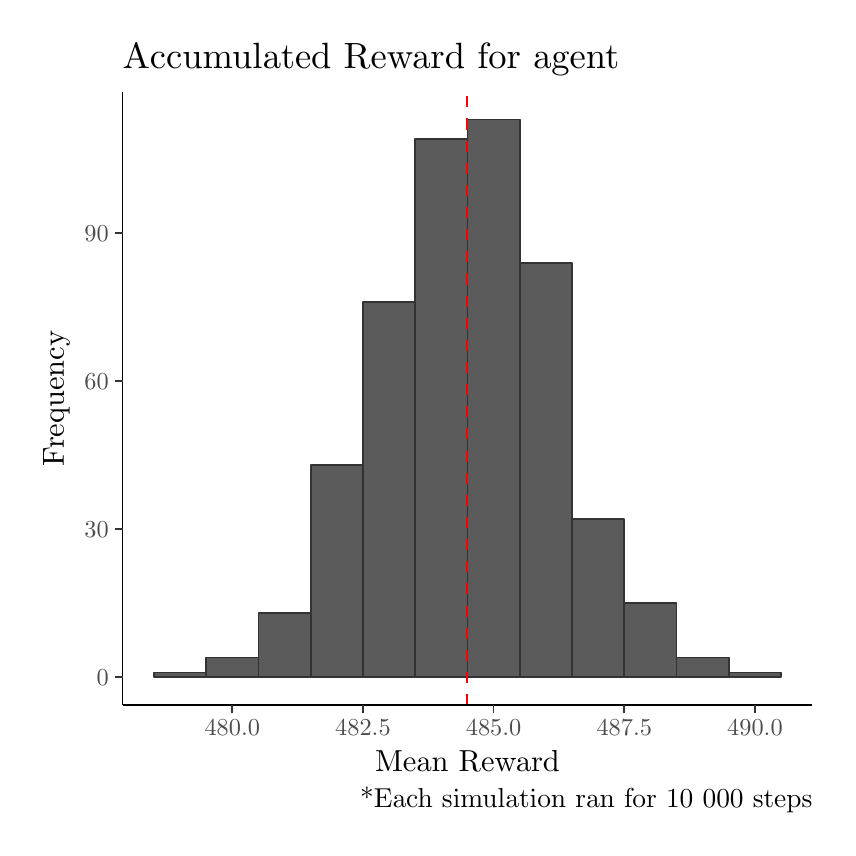
\begin{tikzpicture}[x=1pt,y=1pt]
\definecolor{fillColor}{RGB}{255,255,255}
\path[use as bounding box,fill=fillColor,fill opacity=0.00] (0,0) rectangle (289.08,289.08);
\begin{scope}
\path[clip] (  0.00,  0.00) rectangle (289.08,289.08);
\definecolor{drawColor}{RGB}{255,255,255}
\definecolor{fillColor}{RGB}{255,255,255}

\path[draw=drawColor,line width= 0.6pt,line join=round,line cap=round,fill=fillColor] (  0.00,  0.00) rectangle (289.08,289.08);
\end{scope}
\begin{scope}
\path[clip] ( 34.27, 44.27) rectangle (283.58,265.94);
\definecolor{fillColor}{RGB}{255,255,255}

\path[fill=fillColor] ( 34.27, 44.27) rectangle (283.58,265.94);
\definecolor{drawColor}{gray}{0.20}
\definecolor{fillColor}{RGB}{51,51,51}

\path[draw=drawColor,line width= 0.6pt,line join=round,fill=fillColor,fill opacity=0.80] ( 45.60, 54.35) rectangle ( 64.49, 56.13);

\path[draw=drawColor,line width= 0.6pt,line join=round,fill=fillColor,fill opacity=0.80] ( 64.49, 54.35) rectangle ( 83.37, 61.48);

\path[draw=drawColor,line width= 0.6pt,line join=round,fill=fillColor,fill opacity=0.80] ( 83.37, 54.35) rectangle (102.26, 77.53);

\path[draw=drawColor,line width= 0.6pt,line join=round,fill=fillColor,fill opacity=0.80] (102.26, 54.35) rectangle (121.15,131.03);

\path[draw=drawColor,line width= 0.6pt,line join=round,fill=fillColor,fill opacity=0.80] (121.15, 54.35) rectangle (140.04,189.88);

\path[draw=drawColor,line width= 0.6pt,line join=round,fill=fillColor,fill opacity=0.80] (140.04, 54.35) rectangle (158.92,248.74);

\path[draw=drawColor,line width= 0.6pt,line join=round,fill=fillColor,fill opacity=0.80] (158.92, 54.35) rectangle (177.81,255.87);

\path[draw=drawColor,line width= 0.6pt,line join=round,fill=fillColor,fill opacity=0.80] (177.81, 54.35) rectangle (196.70,204.15);

\path[draw=drawColor,line width= 0.6pt,line join=round,fill=fillColor,fill opacity=0.80] (196.70, 54.35) rectangle (215.59,111.42);

\path[draw=drawColor,line width= 0.6pt,line join=round,fill=fillColor,fill opacity=0.80] (215.59, 54.35) rectangle (234.47, 81.10);

\path[draw=drawColor,line width= 0.6pt,line join=round,fill=fillColor,fill opacity=0.80] (234.47, 54.35) rectangle (253.36, 61.48);

\path[draw=drawColor,line width= 0.6pt,line join=round,fill=fillColor,fill opacity=0.80] (253.36, 54.35) rectangle (272.25, 56.13);
\definecolor{drawColor}{RGB}{255,0,0}

\path[draw=drawColor,line width= 0.6pt,dash pattern=on 4pt off 4pt ,line join=round] (158.82, 44.27) -- (158.82,265.94);
\end{scope}
\begin{scope}
\path[clip] (  0.00,  0.00) rectangle (289.08,289.08);
\definecolor{drawColor}{RGB}{0,0,0}

\path[draw=drawColor,line width= 0.6pt,line join=round] ( 34.27, 44.27) --
	( 34.27,265.94);
\end{scope}
\begin{scope}
\path[clip] (  0.00,  0.00) rectangle (289.08,289.08);
\definecolor{drawColor}{gray}{0.30}

\node[text=drawColor,anchor=base east,inner sep=0pt, outer sep=0pt, scale=  0.88] at ( 29.32, 51.32) {0};

\node[text=drawColor,anchor=base east,inner sep=0pt, outer sep=0pt, scale=  0.88] at ( 29.32,104.82) {30};

\node[text=drawColor,anchor=base east,inner sep=0pt, outer sep=0pt, scale=  0.88] at ( 29.32,158.32) {60};

\node[text=drawColor,anchor=base east,inner sep=0pt, outer sep=0pt, scale=  0.88] at ( 29.32,211.82) {90};
\end{scope}
\begin{scope}
\path[clip] (  0.00,  0.00) rectangle (289.08,289.08);
\definecolor{drawColor}{gray}{0.20}

\path[draw=drawColor,line width= 0.6pt,line join=round] ( 31.52, 54.35) --
	( 34.27, 54.35);

\path[draw=drawColor,line width= 0.6pt,line join=round] ( 31.52,107.85) --
	( 34.27,107.85);

\path[draw=drawColor,line width= 0.6pt,line join=round] ( 31.52,161.35) --
	( 34.27,161.35);

\path[draw=drawColor,line width= 0.6pt,line join=round] ( 31.52,214.85) --
	( 34.27,214.85);
\end{scope}
\begin{scope}
\path[clip] (  0.00,  0.00) rectangle (289.08,289.08);
\definecolor{drawColor}{RGB}{0,0,0}

\path[draw=drawColor,line width= 0.6pt,line join=round] ( 34.27, 44.27) --
	(283.58, 44.27);
\end{scope}
\begin{scope}
\path[clip] (  0.00,  0.00) rectangle (289.08,289.08);
\definecolor{drawColor}{gray}{0.20}

\path[draw=drawColor,line width= 0.6pt,line join=round] ( 73.93, 41.52) --
	( 73.93, 44.27);

\path[draw=drawColor,line width= 0.6pt,line join=round] (121.15, 41.52) --
	(121.15, 44.27);

\path[draw=drawColor,line width= 0.6pt,line join=round] (168.37, 41.52) --
	(168.37, 44.27);

\path[draw=drawColor,line width= 0.6pt,line join=round] (215.59, 41.52) --
	(215.59, 44.27);

\path[draw=drawColor,line width= 0.6pt,line join=round] (262.80, 41.52) --
	(262.80, 44.27);
\end{scope}
\begin{scope}
\path[clip] (  0.00,  0.00) rectangle (289.08,289.08);
\definecolor{drawColor}{gray}{0.30}

\node[text=drawColor,anchor=base,inner sep=0pt, outer sep=0pt, scale=  0.88] at ( 73.93, 33.26) {480.0};

\node[text=drawColor,anchor=base,inner sep=0pt, outer sep=0pt, scale=  0.88] at (121.15, 33.26) {482.5};

\node[text=drawColor,anchor=base,inner sep=0pt, outer sep=0pt, scale=  0.88] at (168.37, 33.26) {485.0};

\node[text=drawColor,anchor=base,inner sep=0pt, outer sep=0pt, scale=  0.88] at (215.59, 33.26) {487.5};

\node[text=drawColor,anchor=base,inner sep=0pt, outer sep=0pt, scale=  0.88] at (262.80, 33.26) {490.0};
\end{scope}
\begin{scope}
\path[clip] (  0.00,  0.00) rectangle (289.08,289.08);
\definecolor{drawColor}{RGB}{0,0,0}

\node[text=drawColor,anchor=base,inner sep=0pt, outer sep=0pt, scale=  1.10] at (158.92, 20.18) {Mean Reward};
\end{scope}
\begin{scope}
\path[clip] (  0.00,  0.00) rectangle (289.08,289.08);
\definecolor{drawColor}{RGB}{0,0,0}

\node[text=drawColor,rotate= 90.00,anchor=base,inner sep=0pt, outer sep=0pt, scale=  1.10] at ( 13.08,155.11) {Frequency};
\end{scope}
\begin{scope}
\path[clip] (  0.00,  0.00) rectangle (289.08,289.08);
\definecolor{drawColor}{RGB}{0,0,0}

\node[text=drawColor,anchor=base west,inner sep=0pt, outer sep=0pt, scale=  1.32] at ( 34.27,274.49) {Accumulated Reward for agent};
\end{scope}
\begin{scope}
\path[clip] (  0.00,  0.00) rectangle (289.08,289.08);
\definecolor{drawColor}{RGB}{0,0,0}

\node[text=drawColor,anchor=base east,inner sep=0pt, outer sep=0pt, scale=  0.99] at (283.58,  7.44) {*Each simulation ran for 10 000 steps};
\end{scope}
\end{tikzpicture}
